\documentclass[./Report_main.tex]{subfiles}
\graphicspath{ ./ }
\begin{comment}
If you want a box around your answer and that answer is an
equation then use \boxed{$$ equation $$} 

if you want to indent a block of text:
\begin{adjustwidth}{cm of right indent}{cm of left indent}
% paragraph to be indented
\end{adjustwidth}

if you just want one indent for one line 
use \indent per intended indent per line

A sections numbers automatically, so if the number of 
the problem is out of order it would be easier to 
just indent and bold the sections and subsections
and not use the \section{} kind of commands

\newpage makes a new page

$normal math mode$
$$Special math mode$$

to include an image use
\includegraphics{image_name}
image_name is the file name (.png) without the extension. The file
name cannot have any spaces or any periods other than the one before
the file extension.

To include a codeblock use
\begin{lstlisting}
ExampleCode(blah, blah)
{
	it does tabbing and everything;
	for (coloring of major languages like java){
		add the folloing to the \lstset tuple:
			language=<name_of_language>;
	}
}
\end{lstlisting}

\end{comment}


\begin{document}

%\tableofcontents

%\thispagestyle{empty}
%\newpage
% If you want to change how the subsubsection's are numbered
%\renewcommand{\thesubsection}{\thesection.\alph{subsection}.} 

%\setcounter{page}{0}
\chapter{Architectural Design}
\section{block diagram}
\subsection{Translation process}
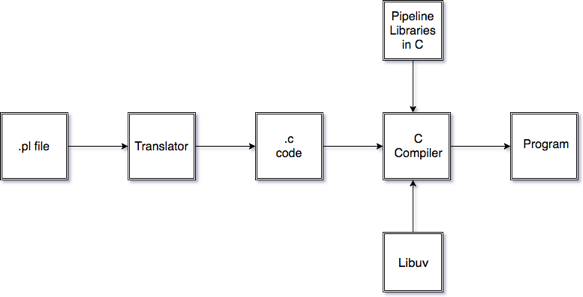
\includegraphics[scale = 0.5]{block_1.png}\\
\subsection{Inside the translator}
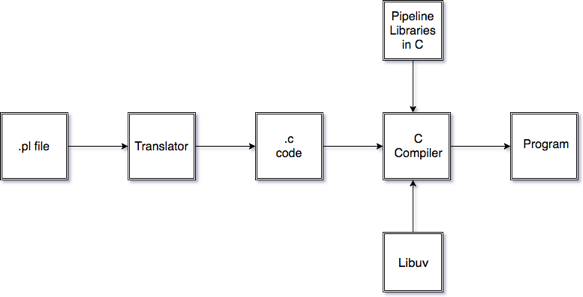
\includegraphics[scale = 0.5]{block_2.png}\\
\section{interface}
\section{implementation responsibility}
%\section{}
%\subsection{Identifiers}
%\subsubsection{}
%\subsection{subsection}
%\subsubsection{subsubsection}
\end{document}

